% \phantomsection
% \manualmark
% \markboth{\spacedlowsmallcaps{Summary}}{\spacedlowsmallcaps{Summary}}
% \addcontentsline{toc}{chapter}{\tocEntry{Summary}}

\phantomsection
\manualmark
\markboth{\spacedlowsmallcaps{Appendix: CrowdTruth Metrics V.2.0}}{\spacedlowsmallcaps{Appendix: CrowdTruth Metrics V.2.0}}
\addcontentsline{toc}{chapter}{\tocEntry{Appendix: CrowdTruth Metrics V.2.0}}{\protect\setcounter{tocdepth}{1}}

\renewcommand{\thesection}{\Alph{section}}

\appendix

\chapter*{Appendix: CrowdTruth Metrics V.2.0}

In this appendix, we present version 2.0 of the CrowdTruth methodology and metrics, that capture and interpret inter-annotator disagreement in crowdsourcing. The novelty in the current version of CrowdTruth is modeling the inter-dependency between the three main components of a crowdsourcing system -- worker, input data, and annotation. The goal of the metrics is to capture the degree of ambiguity in each of these three components. The metrics are available online at \url{https://github.com/CrowdTruth/CrowdTruth-core}.

This chapter is based on the technical report \textit{CrowdTruth 2.0: Quality Metrics for Crowdsourcing with Disagreement}, co-authored by Oana Inel, Benjamin Timmermans, Lora Aroyo and Chris Welty~\cite{dumitrache2018crowdtruth}.


\section{CrowdTruth Methodology}
\label{app:ct2.0}

In previous work~\cite{aroyo2015truth}, we proposed the \textbf{CrowdTruth methodology} as an alternative approach for crowdsourcing ground truth data that, instead of enforcing agreement between annotators, captures the ambiguity inherent in semantic annotation through the use of disagreement-aware metrics for aggregating crowdsourcing responses. The CrowdTruth methodology consists of a set of quality metrics and best practices to aggregate inter-annotator agreement such that ambiguity in the task is preserved. The methodology uses the triangle of disagreement model (based on the triangle reference \cite{knowlton1966definition}) to represent the crowdsourcing system and its three main components -- input media units, workers, and annotations (Figure~\ref{fig:tor}). Based on this model, the CrowdTruth methodology calculates quality metrics for workers, media units and annotations.

 \begin{figure}[!bth]
 	\centering
 		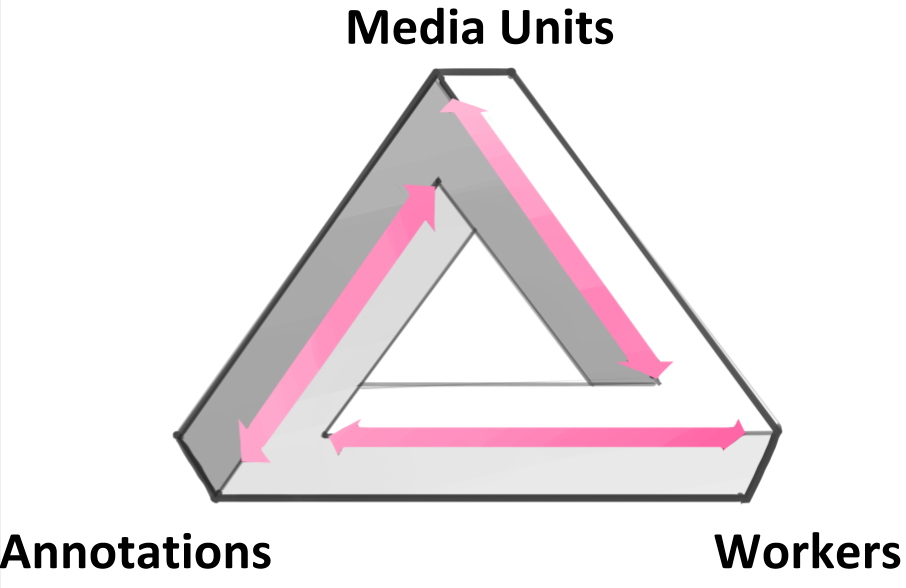
\includegraphics[width=0.5\linewidth]{img/triangle.png}
 	\caption{Triangle of Disagreement}
 	\label{fig:tor}
 \end{figure}


The triangle model also expresses how ambiguity in any of the corners disseminates and influences the other components of the triangle. For example, an unclear sentence or an ambiguous annotation scheme would cause more disagreement between workers \cite{aroyo2014threesides}, and thus, both need to be accounted for when measuring the quality of the workers. Based on this observation, we introduce \textbf{version 2.0 of CrowdTruth metrics} -- a set of metrics that capture and interpret inter-annotator disagreement in crowdsourcing annotation tasks. As opposed to the first version of the metrics, published in~\cite{inel2014crowdtruth}, the current version models the \textit{inter-dependency between the three main components of a crowdsourcing system -- worker, input data, and annotation}. So for example, the quality of a worker is weighted by the quality of the media units the worker has annotated, and the quality of the annotations in the task. This update is based on the intuition that disagreement caused by low quality workers should not be interpreted as the data being ambiguous, but also that ambiguous input data should not be interpreted as due to the low quality of the workers.

The following sections describe how to formalize the output from the crowd into \textbf{annotation vectors} (Section~\ref{app:vec}), and how to calculate quality scores over the annotation vectors using \textbf{disagreement metrics} (Section~\ref{app:metrics}). The code of the implementation of the metrics is available on the CrowdTruth Github.\footnote{\url{https://github.com/CrowdTruth/CrowdTruth-core}} The 2.0 version of the metrics has already been applied in Chapters~\ref{chap:od-rel-ex} and~\ref{chap:frames}, as well as to a number of use cases not discussed in this thesis, e.g. topic relevance~\cite{inel2018studying}.


\section{Building the Annotation Vectors}
\label{app:vec}

\begin{figure}[!htb]
 	\centering
 	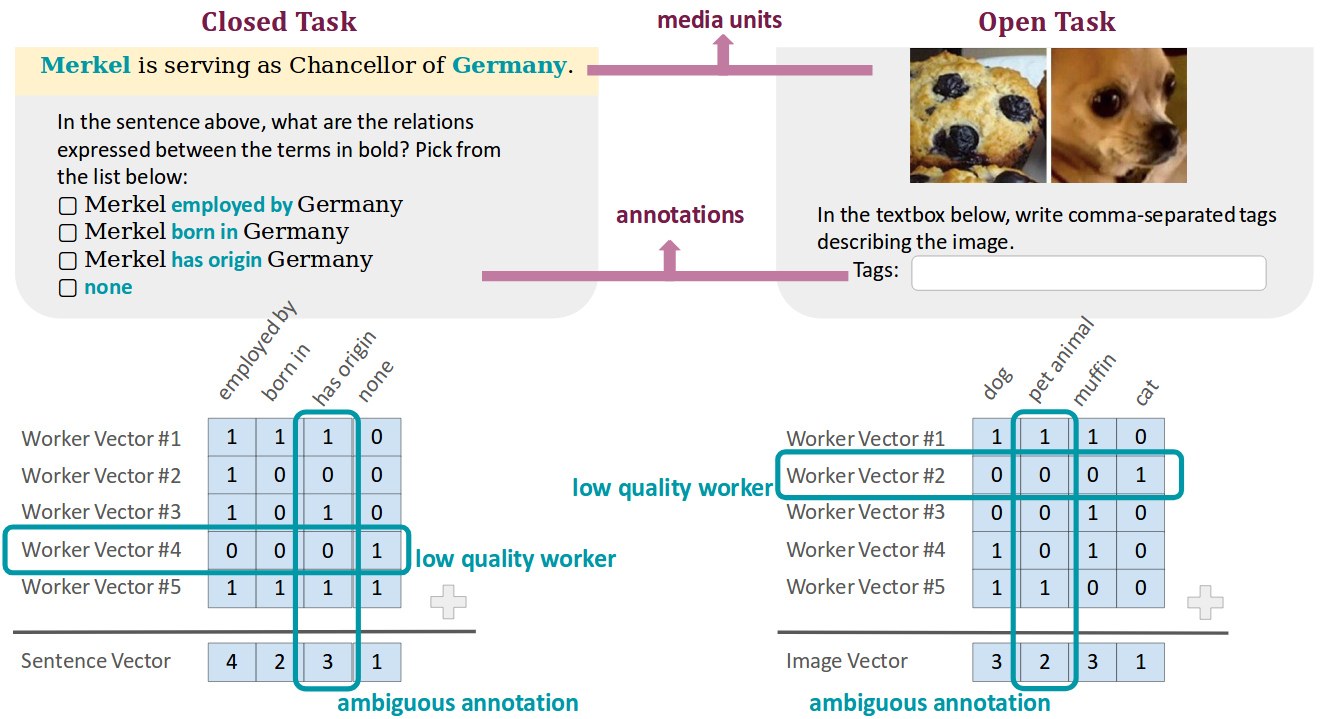
\includegraphics[width=\linewidth]{img/closed_open_task.png}
 	\caption{Example closed and open tasks, together with the vector representations of the crowd answers.}
 	\label{fig:tasks}
 \end{figure}

In order to measure the quality of the crowdsourced data, we need to formalize crowd annotations into a \textbf{vector space representation}. For \emph{closed tasks}, the annotation vector contains the given answer options in the task template, which the crowd can choose from. For example, the template of a \emph{closed task} can be composed of a multiple choice question, which appears as a list checkboxes or radio buttons, thus, having a finite list of options to choose from. Figure~\ref{fig:tasks} shows an example of a closed and an open task, indicating also what the media units and annotations are for both cases.

While for \emph{closed tasks} the number of elements in the annotation vector is known in advance, for \emph{open-ended tasks} the number of elements in the annotation vector can only be determined when all the judgments for a media unit have been gathered. An example of such a task can be highlighting words or word phrases in a sentence, or as an input text field where the workers can introduce keywords. In this case the answer space is composed of all the unique keywords from all the workers that solved that media unit. As a consequence, all the media units in a closed task have the same answers space, while for open-ended tasks the answer space is different across all the media units. Although the answer space for open-ended tasks is not known from the beginning, it still can be further processed in a finite answer space.

In the annotation vector, each answer option is a boolean value, showing whether the worker annotated that answer or not. This allows the annotations of each worker on a given media unit to be aggregated, resulting in a \textbf{media unit vector} that represents for each option how often it was annotated. Figure~\ref{fig:tasks} shows how the worker and media unit vectors are formed for both a closed and an open task.

\section{Disagreement Metrics}
\label{app:metrics}

Using the vector representations, we calculate three core metrics that capture the \textbf{media unit quality}, \textbf{worker quality} and \textbf{annotation quality}. These metrics are mutually dependent (e.g. the media unit quality is weighted by the annotation quality and worker quality), based on the idea from the triangle of disagreement that ambiguity in any of the corners disseminates and influences the other components of the triangle. The mutual dependence requires an iterative dynamic programming approach, calculating the metrics in a loop until convergence is reached. All the metrics have scores in the $[0,1]$ interval, with $0$ meaning low quality and $1$ meaning high quality. Before starting the iterative dynamic programming approach, the quality metrics are initialized with $1$. % as we assume that workers, media units and annotations have maximum quality 

To define the CrowdTruth metrics, we introduce the following notation:
\begin{itemize}
\item $workers(u):$ all workers that annotate media unit $u$;
\item $units(i):$ all input media units annotated by worker $i$;
\item worker vector $\vec{w}_{i, u}:$ annotations of worker $i$ on media unit $u$ as a binary vector;
\item media unit vector $\vec{u} = \sum\limits_{i \in workers(u)} \vec{w}_{i,u}$: the sum of all worker vectors $\vec{w}_{i,u}$ for a given media unit $u$.
\end{itemize}

To calculate agreement between 2 workers on the same media unit, we compute the cosine similarity over the 2 worker vectors. In order to reflect the dependency of the agreement on the degree of clarity of the annotations, we compute $WCos$, the weighted version of the cosine similarity. The Annotation Quality Score (AQS), which will be described in more detail at the end of the section, is used as the weight. For open-ended tasks, where annotation quality cannot be calculated across multiple media units, we consider annotation quality equal to 1 (the maximum value) in all cases. Given 2 worker vectors, $\vec{x}$ and $\vec{\vec{y}}$ on the same media unit, the formula for the weighted cosine score is:

\begin{align}
WCos(\vec{x}, \vec{y}) = & \dfrac{\sum\limits_{a} \vec{x} (a) \; \vec{y} (a) \;  AQS(a)}{\sqrt{(\sum\limits_{a} \vec{x}(a)^2 \; AQS(a)) \; (\sum\limits_{a} \vec{y}(a)^2 \; AQS(a))}}, \\
& \forall a \text{ - annotation}. \nonumber
\end{align}

The \textbf{Media Unit Quality Score (UQS)} expresses the overall worker agreement over one media unit. This metric is a generalized definition of the \textit{sentence quality score} described in Chapter~\ref{sec:frame-metrics}. Given an input media unit $u$, $UQS(u)$ is computed as the average cosine similarity between all worker vectors, weighted by the worker quality ($WQS$) and annotation quality ($AQS$). Through the weighted average, workers and annotations with lower quality will have less of an impact on the final score. The formula used in its calculation is:

\begin{align}
UQS(u) = & \dfrac{\sum\limits_{i, j} WCos(\vec{w}_{i,u} , \vec{w}_{j,u}) \; WQS(i) \; WQS(j)}{\sum\limits_{i,j} WQS(i) \; WQS(j)}, \\
& \forall i, j \in workers(u), i \neq j. \nonumber
\end{align}

%\subsection{Worker Quality Score (WQS)}
The \textbf{Worker Quality Score (WQS)} measures the overall agreement of one crowd worker with the other workers. Given a worker $i$, $WQS(i)$ is the product of 2 separate metrics - the worker-worker agreement $WWA(i)$ and the worker-media unit agreement $WUA(i)$:

\begin{align}
WQS(i) = WUA(i) \; WWA(i) .
\end{align}

%Worker-Worker Agreement
The \textbf{Worker-Worker Agreement (WWA)} for a given worker $i$ measures the average pairwise agreement between $i$ and all other workers, across all media units they annotated in common, indicating how close a worker performs compared to workers solving the same task.  The metric gives an indication as to whether there are consistently like-minded workers. This is useful for identifying communities of thought. $WWA(i)$ is the average cosine distance between the annotations of a worker $i$ and all other workers that have worked on the same media units as worker $i$, weighted by the worker and annotation qualities. Through the weighted average, workers and annotations with lower quality will have less of an impact on the final score of the given worker.

\begin{align}
 WWA(i) = & \dfrac{ \sum\limits_{j, u} WCos(\vec{w}_{i,u} , \vec{w}_{j,u}) \; WQS(j) \; UQS(u) }{ \sum\limits_{j, u} WQS(j) \; UQS(u) }, \\
& \forall j \in workers(u \in units(i)), i \neq j . \nonumber
\end{align}

%Worker-Media Unit Agreement
The \textbf{Worker-Media Unit Agreement (WUA)} measures the similarity between the annotations of a worker and the aggregated annotations of the rest of the workers. In contrast to the $WWA$ which calculates agreement with individual workers, $WUA$ calculates the agreement with the consensus over all workers. $WUA(i)$ is the average cosine distance between the annotations of a worker $i$ and all annotations for the media units they have worked on, weighted by the media unit ($UQS$) and annotation quality ($AQS$). Through the weighted average, media units and annotations with lower quality will have less of an impact on the final score.

\begin{align}
WUA(i) = & \dfrac{\sum\limits_{u \in units(i)} WCos(\vec{w}_{i,u} , \vec{u} - \vec{w}_{i,u}) \; UQS(u)}{\sum\limits_{u \in units(i)} UQS(u)}.
\end{align}

The \textbf{Annotation Quality Score (AQS)} measures the agreement over an annotation in all media units that it appears. Therefore, it is only applicable to closed tasks, where the same annotation set is used for all input media units. This metric is a generalized definition of the \textit{frame quality score} described in Chapter~\ref{sec:frame-metrics}. AQS is based on $P_a(i | j)$, the probability that if a worker $j$ annotates $a$ in a media unit, worker $i$ will also annotate it.

\begin{align}
P_a(i | j) = & \frac{ \sum\limits_{u} \vec{w}_{i,u}(a) \; \vec{w}_{j,u}(a) \; UQS(u)}{ \sum\limits_{u} \vec{w}_{j, u}(a) \;  UQS(u) }, \\
& \forall u \in units(i) \cap units(j). \nonumber
\end{align}

Given an annotation $a$, $AQS(a)$ is the weighted average of $P_a(i | j)$ for all possible pairs of workers $i$ and $j$. Through the weighted average, input media units and workers with lower quality will have less of an impact on the final score of the annotation.

\begin{align}
AQS(a) = & \dfrac{ \sum\limits_{i,j} WQS(i) \; WQS(j) \; P_a(i | j) }{ \sum\limits_{i,j} WQS(i) \; WQS(j) }, \\
& \forall i, j \text{ workers, }  i \neq j . \nonumber
\end{align}

The formulas for media unit, worker and annotation quality are all mutually dependent. To calculate them, we apply an iterative dynamic programming approach. First, we initialize each quality metric with the score for maximum quality (i.e. equal to 1). Then we repeatedly re-calculate the quality metrics until each of the values are stabilized. This is assessed by calculating the sum of variations between iterations for all quality values, and checking until it drops under a set threshold $t$.

The final metric we calculate is the \textbf{Media Unit - Annotation Score (UAS)} -- the degree of clarity with which an annotation is expressed in a unit. This metric is a generalized definition of the \textit{sentence-relation score} described in Chapter~\ref{sec:chap4_metrics}, and the \textit{frame-sentence score} described in Chapter~\ref{sec:frame-metrics}. Given an annotation $a$ and a media unit $u$, $UAS(u, a)$ is the ratio of the number of workers that picked annotation $u$ over all workers that annotated the unit, weighted by the worker quality:

\begin{align}
UAS(u, a) = \dfrac{ \sum\limits_{i \in workers(u)} \vec{w}_{i,u}(a) \; WQS(i) }{ \sum\limits_{i \in workers(u)} WQS(i) }.
\end{align}


\section*{Acknowledgments}

We would like to thank Markus de Jong, Evgeny Krivosheev and Panagiotis Mavridis for their valuable feedback in improving the mathematical notation and readability of the chapter. 